\subsubsection{Properties, Parcels and Campaign Coverage}
\label{sec:conceptual-properties}
Property and HarvestCampaign belong independently to a Workspace. Parcel is an
optional reusable division of a Property. CampaignCoverage links a campaign to
one or more whole properties or selected parcels, allowing a campaign to span
several properties without duplicating their records.
Figure~\ref{fig:er-properties-campaigns} shows the coverage relationships.

\begin{figure}[!htbp]
\centering
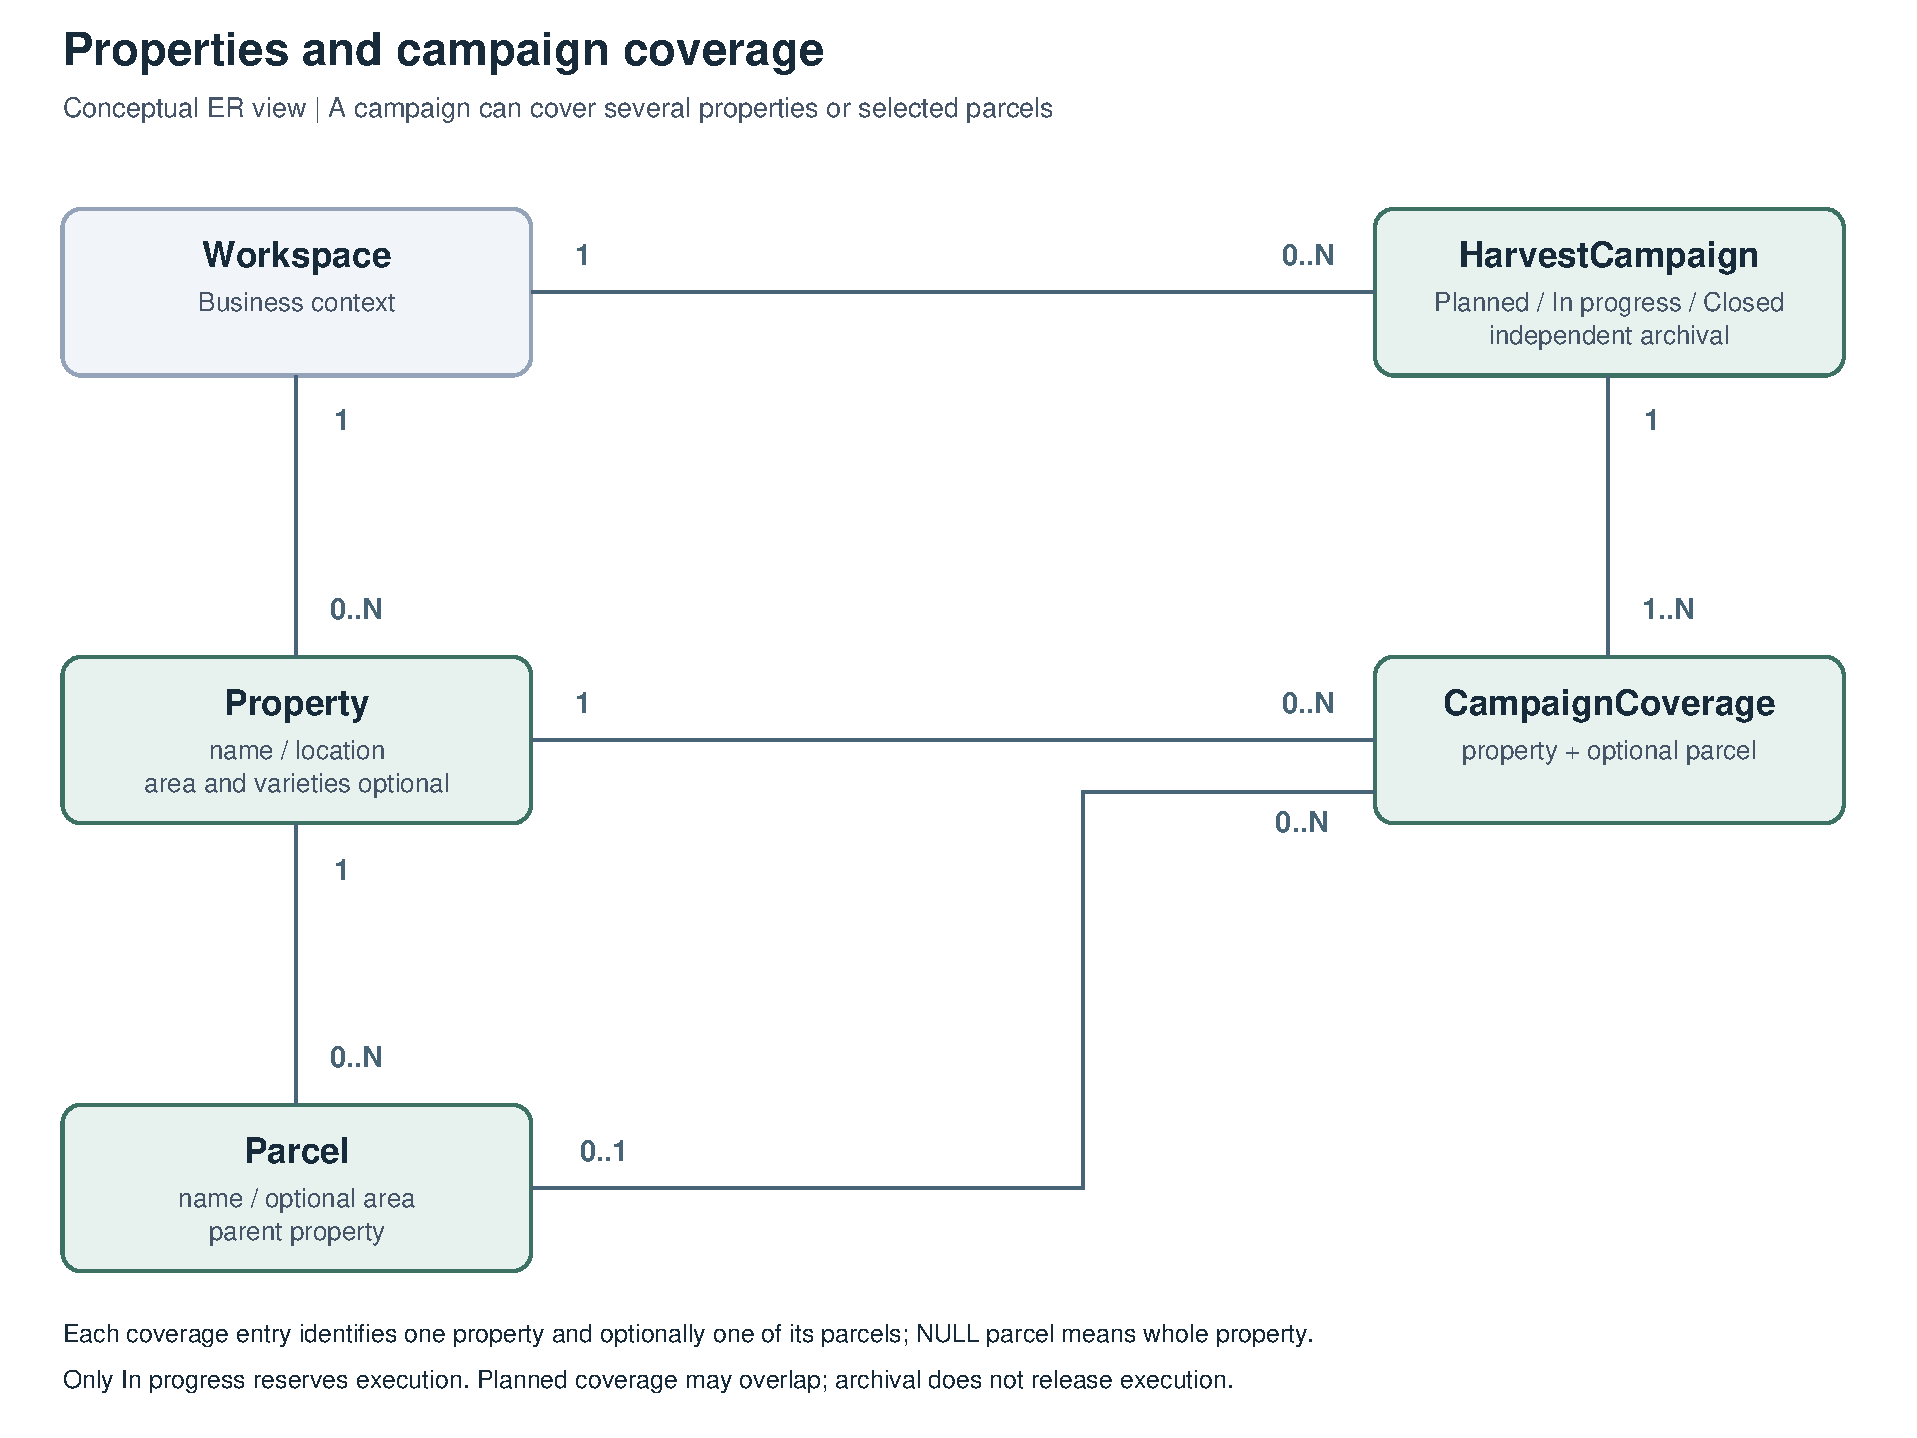
\includegraphics[width=\textwidth]{figures/er-properties-campaigns.pdf}
\caption{Properties, optional parcels and campaign coverage. A coverage entry always identifies a property and optionally one of its parcels.}
\label{fig:er-properties-campaigns}
\end{figure}

A coverage entry always identifies a property and optionally one of its parcels;
an absent parcel denotes whole-property coverage. Operational area references use
the same representation. This preserves the difference between property-level
and parcel-level information when divisions are added later.

HarvestCampaign stores planned start, actual start and actual end separately.
Lifecycle and archival are separate fields because execution/closure govern dates,
while archival controls normal-list visibility. CampaignCoverage is the set against
which start/reopening and In progress coverage changes enforce
\hyperref[br:008]{\identifier{BR-008}}. This cross-record constraint needs transactional
validation; the ER relation alone cannot enforce exclusive execution.
